\documentclass[a4paper,11pt,singlespacing]{article}

\usepackage{setspace}
\usepackage[utf8]{inputenc}
\usepackage[T1]{fontenc}
\usepackage{graphicx}
\usepackage{color}
\usepackage{hyperref}
\usepackage{listings,xcolor}

\renewcommand{\figurename}{Abbildung}

\graphicspath{ {./images/} }

\title{Hacking von I LOCK IT}
\author{Marius Würstle}
\date{\today}

\begin{document}
	\setlength{\parindent}{0ex}
	\maketitle
	
	\tableofcontents
	\pagebreak
	
	\section{Motivation}
	
	\section{Grundbegriffe}
		CRCInit
		
	
	\section{Problemstellung}
	
	\section{Sicherheitsanalyse}
	
	\section{Herangehensweisen}
		Meine verschiedenen Ansätze (z.B. App Decodieren, mitschneiden des Datenverkehrs)
			
	\subsection{Bluetooth und Bluetooth Low Energy}
		Bluetooth ist der Industriestandard für die drahtlose Datenübertragung über kurze Distanz. Die Slaves lauschen auf 32 unterschiedlichen Hop-Kanälen, dieser Modus nennt sich Scan-Modus. Der Verbindungsaufbau geht von einem Master Gerät aus und wird mittels einer Inquiry-Nachricht und einer anschließenden Page-Nachricht hergestellt. Falls die Hardware-Adresse(48-Bit lange eindeutige ID) den Geräten bekannt ist wird keine Page Nachricht mehr versendet. In der Page Phase sendet der Master 16 identische Page Nachrichten auf 16 verschiedene Channels. \\
		Bluetooth Low Energy (BLE) wurde für Systeme entwickelt, die auf einem Akku basieren und mit einem möglichst geringen Stromverbrauch funktionieren müssen. Dies wird durch kurze Aktivitätszeiten erreicht, das heißt es wird nur gesendet bzw. gelauscht solange es notwendig ist. Zusätzlich werden die Datenpakete gesammelt und alle zusammen versandt. Darüber hinaus spart die geringe Übertragungsgeschwindigkeit Strom.
		
		\subsubsection{Advertising}
		BLE nutzt 40 verschieden Channels im Bereich von 2402 MHz bis 2480 MHz. Die einzelnen Channels sind 2 MHz voneinander entfernt, davon werden Channel 37, 38 und 39 nur für das Advertisement verwendet. \\
		Die sogenannten Adveritsements sind die Pakete, die von den Peripherie Geräten ausgesendet werden, um auf sich aufmerksam zu machen. Es gibt noch einige Spezifikationen, der einzelnen Advertisment-Pakete, dies würde allerdings den Rahmen der Arbeit sprengen. Meist sind in diesem Paket der Gerätename, die Service UUID und die RSSI (RSSI Pegel und Signalstärke). Falls die 31 Bytes an Advertisement-Data des Pakets nicht ausreichen, um alle Informationen in das Advertiesment Paket zu packen, kann ein Scan-Request gesendet werden. Welcher logischerweise mit den restlichen Daten in einem Scan-Response beantwortet wird. Allerdings muss das Zentrale System die Anfrage auslösen, um die Daten zu bekommen.
		\begin{figure}[ht]
			\centering
			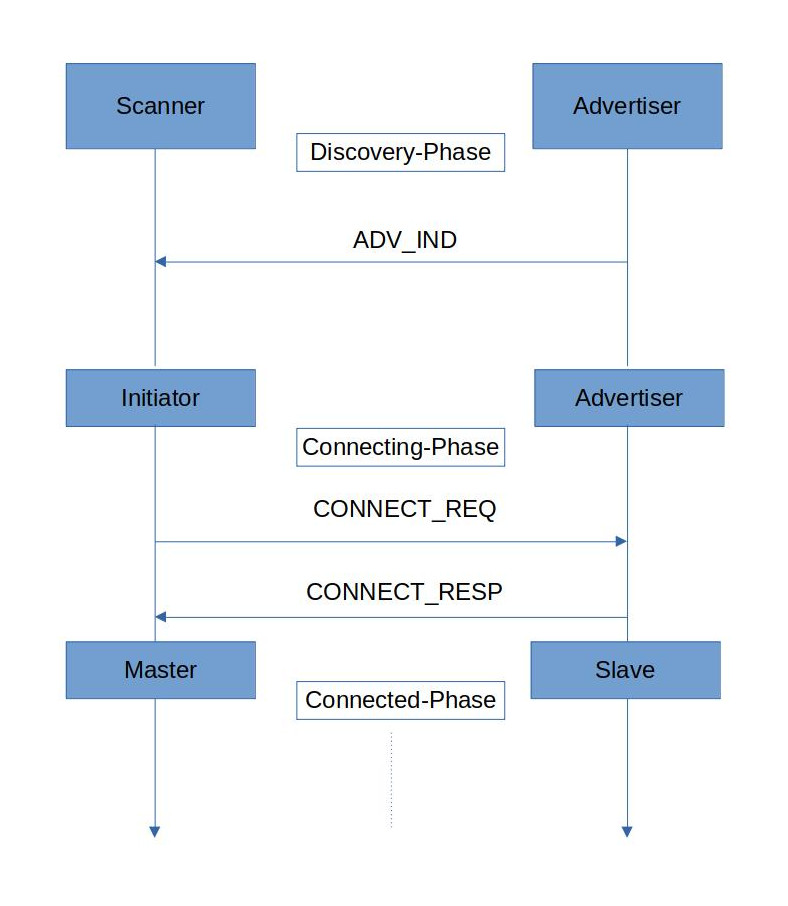
\includegraphics[scale=0.4]{Connection_BLE}
			\caption{Verbindungsaufbau unter BLE}
			\label{connect}
		\end{figure}
		\subsubsection{Discovery-Phase}
		Die Peripherie Geräte senden ihre Advertisement in dieser Phase auf die 3 oben gennanten Channel mit den auch oben genannten Informationen. Hier könnte auch ein Scan-Request getätigt werden.
		\subsubsection{Connection-Phase}
		Der Master wird jetzt "Initiatior" gennannt und antwortet mit einem "CONNECT\_REQ". Dieses Paket beinhaltet die CRCInit, WinSize, WinOffset, das Intervall, die Signalstärke und den Timeout. Nach dem versenden oder dem Erhalt dieses Pakets gelten die Systeme als verbunden.
		\subsubsection{Connected-Phase}
		Nachdem dem Verbindungsaufbau wird der Initiator zum Master und der Advertiser zum Slave und es können Daten ausgetauscht werden. Bei BLE wird dies über dem Linked-Layer gemacht, welcher auch verschlüsselt werden kann.
		
		\subsection{}
	
	\section{Umsetzung}
		
		Eine kleine Anleitung und Erläuterung, wie das Schloss geknackt werden kann.
		
	\section{Fazit/Ausblick}
		Nennung der Sicherheitslücken und Ideen wie man diese verhindern kann.
	
	
	
	
	
	
	https://www.rfwireless-world.com/Terminology/BLE-Connection-Establishment-Procedure.html 20 März 2021
	
\end{document}